\documentclass[book.tex]{subfiles}
\begin{document}
PC performances in the 90s were so overwhelmingly dominated by their CPU that they were simply referred to not by their brand or model but by their Intel chip. If your PC has an Intel 80386SX in it, it was a 386. If it had an Intel 80286, it was a 286. Wolfenstein was target at 386s with degraded performances (yet still playable) on 286s.\\
\\
In order to understand the machine I broke it down in five components part of a pipeline: Input, Cpu, Ram, Video and Audio.\\
 \bigskip
\begin{figure}[H]
\centering
\includegraphics[scale=1.2]{imgs/fun_pipeline.pdf}
%\def\svgscale{1.5}
%\input{imgs/fun_pipeline.pdf_tex}
\caption{Hardware pipeline.}
\label{fig:digraph}
\end{figure}

None of theses part were good for game although some were worse than others:

 \bigskip

\begin{figure}[H]
\centering
\begin{tabularx}{\textwidth}{ X X  }
  \toprule
  \textbf{Stage} & \textbf{Quality} \\ \bottomrule
  RAM & Very Poor \\ 
  Video & Very Poor \\ 
  Audio & Poor \\ 
  Inputs & Good \\ 
  CPU & Poor \\ \bottomrule
\end{tabularx}
\caption{Component quality for a game engine.}  \label{fig:Component quality for a game engine.}
\end{figure}

\footnote{Even though the CPU was powerful it was very good only at something next to useless for a 3D engine: Integer arithmetic.}

Overall, the pipeline offered a lot of resistance: hardware manufacturers had not embraced the game industry yet and it showed a lot. Ever since their inception in the 70s, IBM Personal Computers were designed to display static images and crunch integers. Real-time 3D, fractions and smooth sixty-frames-per-seconds animations were part of the blueprints.

\section{Central Processing Unit}
  \subsection{Overview}
  The ubiquitous CPU manufacturer was Intel with its x86 line of microprocessors.  The machines based on the 80286 released in 1982 were on the decline and progressively replaced by Intel's first 32 bits processor: The 80386. Moore's law was in full swing as can be seen on a mips\footnote{Million Instructions Per Second.} histogram:


\definecolor{skyblue1}{rgb}{0.1,0.624,0.812}


\begin{figure}[H]
\centering
  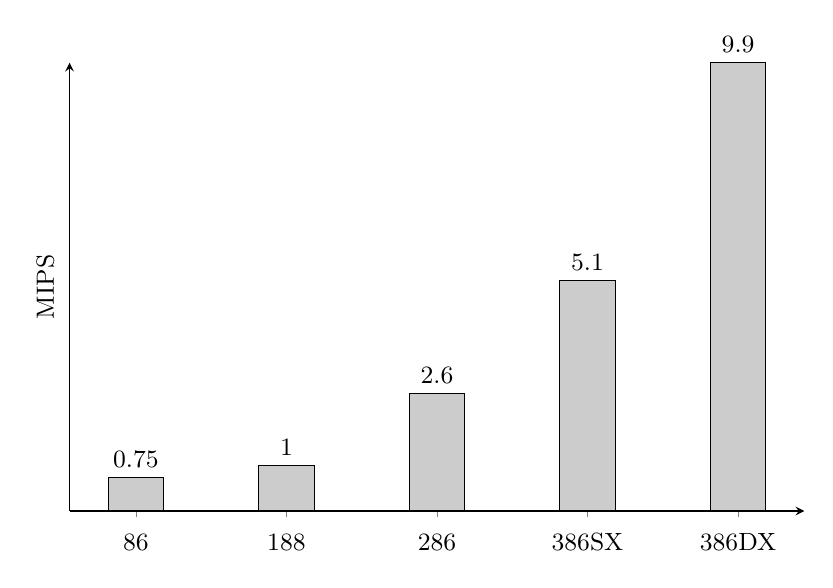
\begin{tikzpicture}[font=\small]
    \begin{axis}[
      width=0.9\textwidth,
      height=0.6\textwidth,
      ybar,
      bar width=20pt,
      ylabel={MIPS},
      ymin=0,
      ytick=\empty,
      xtick=data,
      axis x line=bottom,
      axis y line=left,
      enlarge x limits=0.11,
      symbolic x coords={86,188,286,386SX,386DX},
      xticklabel style={anchor=base,yshift=-\baselineskip},
      nodes near coords={\pgfmathprintnumber\pgfplotspointmeta}
    ]
      \addplot[fill=black!20,draw=black] coordinates {
        (86,0.75)
        (188,1)
        (286,2.6)
        (386SX,5.1)
        (386DX,9.9)
      };
    \end{axis}
    
   \end{tikzpicture}
   \caption{Processor speeds comparison.} \label{fig:mips}
 \end{figure}

 \textbf{\underline{Trivia :}} A modern processor such as the Intel Core i7 3.33 GHz operates at close to 180,000 Mips: Five orders of magnitude faster!

 \bigskip

\textbf{\underline{Trivia :}}  Two other companies were producing Intel clones: AMD and Cyrix. The mediocre performances did not justify the lower cost and as a result they never gathered a significant market share. Interestingly AMD evolved to become a serious challenger while Cyrix merged with National Semiconductor in 1997.

 \bigskip
 
 \textbf{\underline{Trivia :}} The 386SX and 386DX were identical processor. Yet the DX is twice faster than the SX thanks to a data bus between the CPU and the RAM twice as wide (32 bits vs 16 bits) !












  \subsection{Floating Point}
  
   PC 286s and 386s were powerful machines far outperforming any game console on the market. But all that power was not necessarily useful. In order to perform all the trigonometry for a '3D' game, the machines had to keep track of the fractional part of each operations. This is not an issue since the C language offers the types \codeword{float} and \codeword{double} precisely for that.\\
\\
It is important to understand what floating point is and how it works to fully grasp how useful it is when doing maths. \codeword{float} are 32 bits container following the IEEE 754 standard. Their purpose is to store and allow operations on approximation of real numbers. The 32 bits are divided in three sections:\\
\begin{itemize}
  \item One bit S for the sign.
  \item Seven bits E for the exponent.
  \item Twenty four bits for the mantissa.
\end{itemize} 

\begin{figure}[H]
\centering
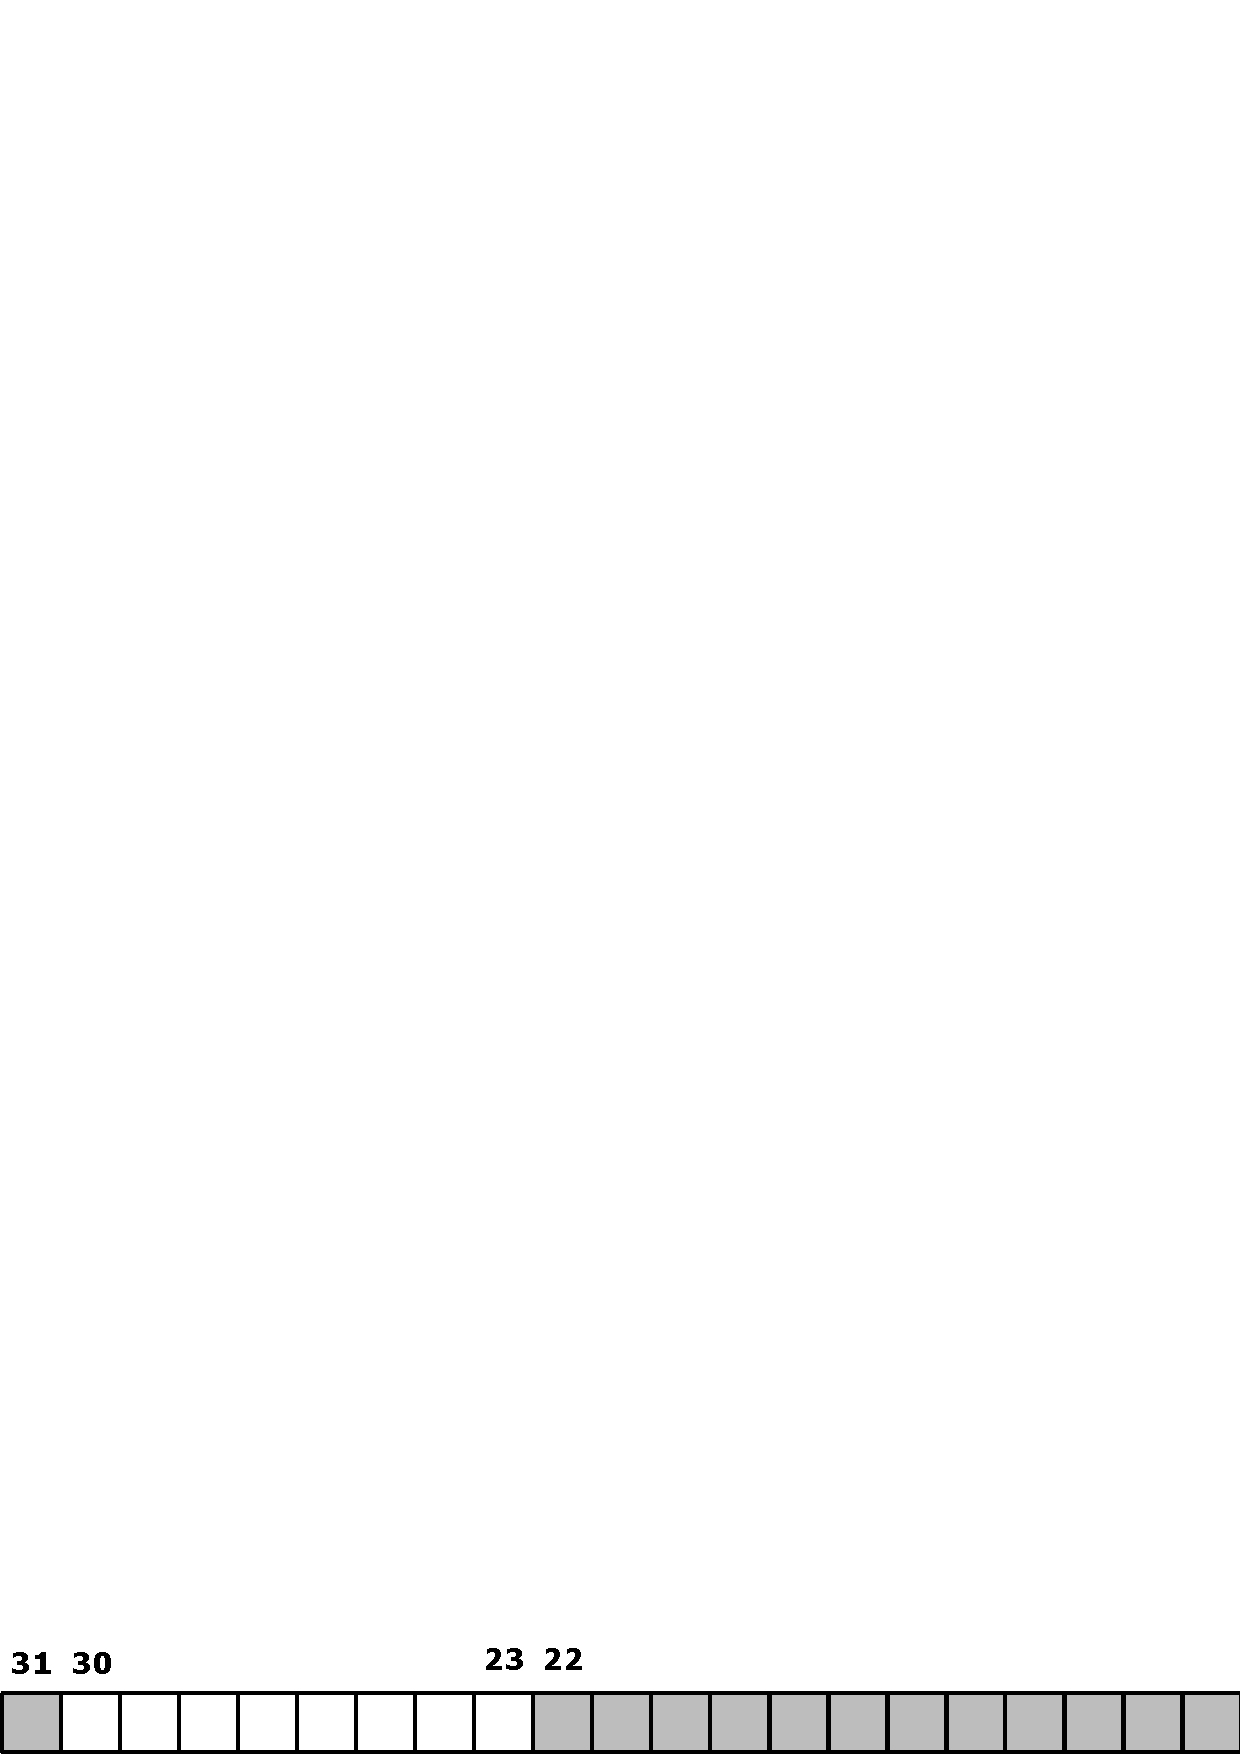
\includegraphics[scale=0.4]{imgs/floating_point_layout.pdf}
\caption{Floating Point internals}
\label{fig:fp_internals}
\end{figure}
  \bigskip



\begin{figure}[H]
\centering
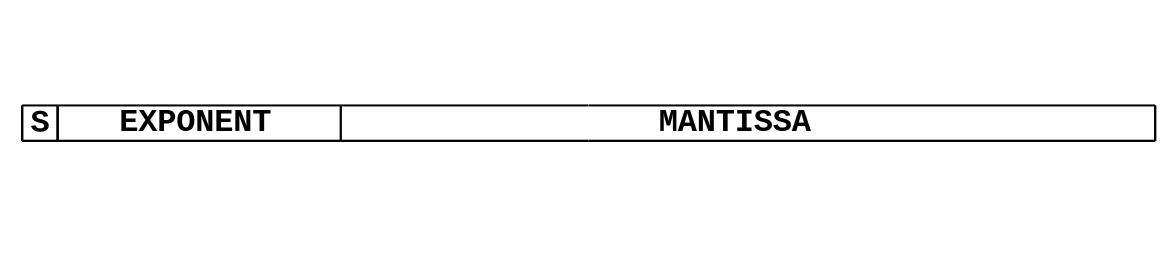
\includegraphics[scale=0.4]{imgs/floating_point_math.pdf}
\caption{Floating Point three sections}
\label{fig:fp_regions}
\end{figure}
  \bigskip  


How numbers are stored and interpreted is usually explained with the formula \ref{eq:fp}).\


\begin{equation}\label{eq:fp}
\large
(-1)^S * 1.M * 2^{(E-127)}
\end{equation}
 
\bigskip  
Although correct, this way to explain floating point usually leaves programmers completely clueless. I blame this ignoble notation for discouraging generations of programmers, scaring them to the point they never looked back to understand how floating point actually works. Fortunately, there is a better way to explain it: Instead of Exponent, think of a floating window between two consecutive power of two integers. And instead of a Mantissa think of an Offset within that window as in Figure \ref{fig:fp_internals}:
  
\begin{figure}[H]
\centering
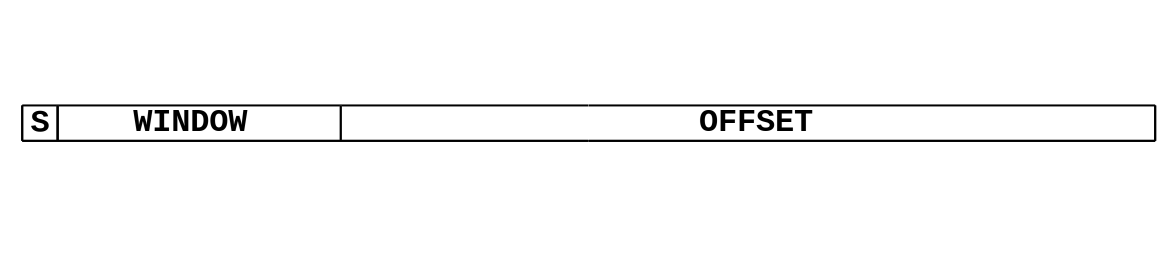
\includegraphics[scale=0.4]{imgs/floating_point_intuitive.pdf}
\caption{Alternative Floating Point internals}
\label{fig:fp_internals}
\end{figure}
  \bigskip  

Figure \ref{fig:fp_internals_window} illustrate how the number 6.1 would be encoded, with the window starting at 4 (and therefore spanning up to next power of two: 8). The offset about half way down the window.

\begin{figure}[H]
\centering
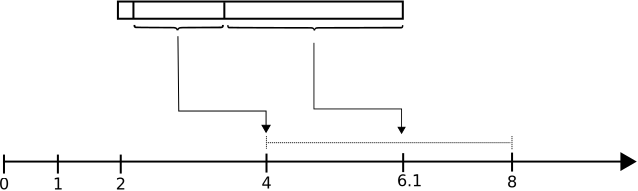
\includegraphics[scale=0.7]{imgs/floating_point_window.pdf}

\caption{Value 6.1 approximated with floating point}
\label{fig:fp_internals_window}
\end{figure}
  \bigskip
  
Here is a detailled example which calculate the floating point representation of the number 3.14.
\begin{itemize}
 \item The number 3.14 is positive  $\rightarrow S=0$.
 \item The number 3.14 is between the power of two 2 and 4 so the floating window must start at $2^1$  $\rightarrow E=128$.
 \item Finally there are $2^{23}$ offsets available so 3.14 is at $\frac{4-3.14}{2} = 0.43 $. The mantissa/offset $\rightarrow M = 2^{23}*0.43 = 4781506$
\end{itemize}

Which in binary translate to:

\begin{itemize}
\item S = 0.
\item E = 10000000
\item M = 1001000111101111000011
\end{itemize}

\begin{figure}[H]
\centering
\includegraphics[scale=0.4]{imgs/floating_point_layout_pi.pdf}
\caption{Floating Point internals}
\label{fig:fp_internals}
\end{figure}
  \bigskip

The value 3.14 is therefore approximated to 3.140000104904175.\\

The corresponding value with the ugly and useless formula:

\begin{equation}
3.14 = (-1)^0 * 1.57 * 2^{(128-127)}
\end{equation}

\bigskip

And finally the graphic representation:\\

\begin{figure}[H]
\centering
\includegraphics[scale=0.7]{imgs/floating_point_window_pi.pdf}

\caption{3.14 window and offset.}
\label{fig:fp_internals}
\end{figure}
  \bigskip

Floating Point are very handy: They can represent very small values and huge ones while keeping track of fractional part of a number and also protecting from overflow by floating the window when necessary.\\
\\
They are neat but computational intensive: In order to add, subtract, multiply or divide two numbers, they have to be expressed with the same window. Which mean converting one number to the representation used by the other usually with higher precision than 32 bits (typically 80 bits on Intel FPUs).\\
\\
This is not a problem when everything is hardwired...but it was a big problem for the 286 and the 386: \emph{They did not have a hardware Floating Point Unit}. Those operations were emulated in software by the compiler and therefore terribly slow. So slow they were not usable for anything real-time. 

  \bigskip

 \textbf{\underline{Trivia :}} Since floating point units where so slow, why did the C language end up with a \codeword{float} and \codeword{double} types ? The machine used to invent the language (PDP-11) did not have a floating point but the manufacturer (DEC) had promised Dennis Ritchie and Ken Thompson the next model would have one\footnote{The Development of the C Language by Dennis M. Ritchie}. Being astronomy enthusiasts they decided to add those two types to their language. Had they decided not to, C and C++ would have never enjoyed the same popularity!

\bigskip  
\break
\textbf{\underline{Trivia :}} Some PCs did have hardware FPU. Intel sold what was marked as "Math CoProcessor". Intented to scientists, performances were average, price outrageous and sales mediocre :\\
\begin{figure}[H]
\centering
  \shadowbox{
      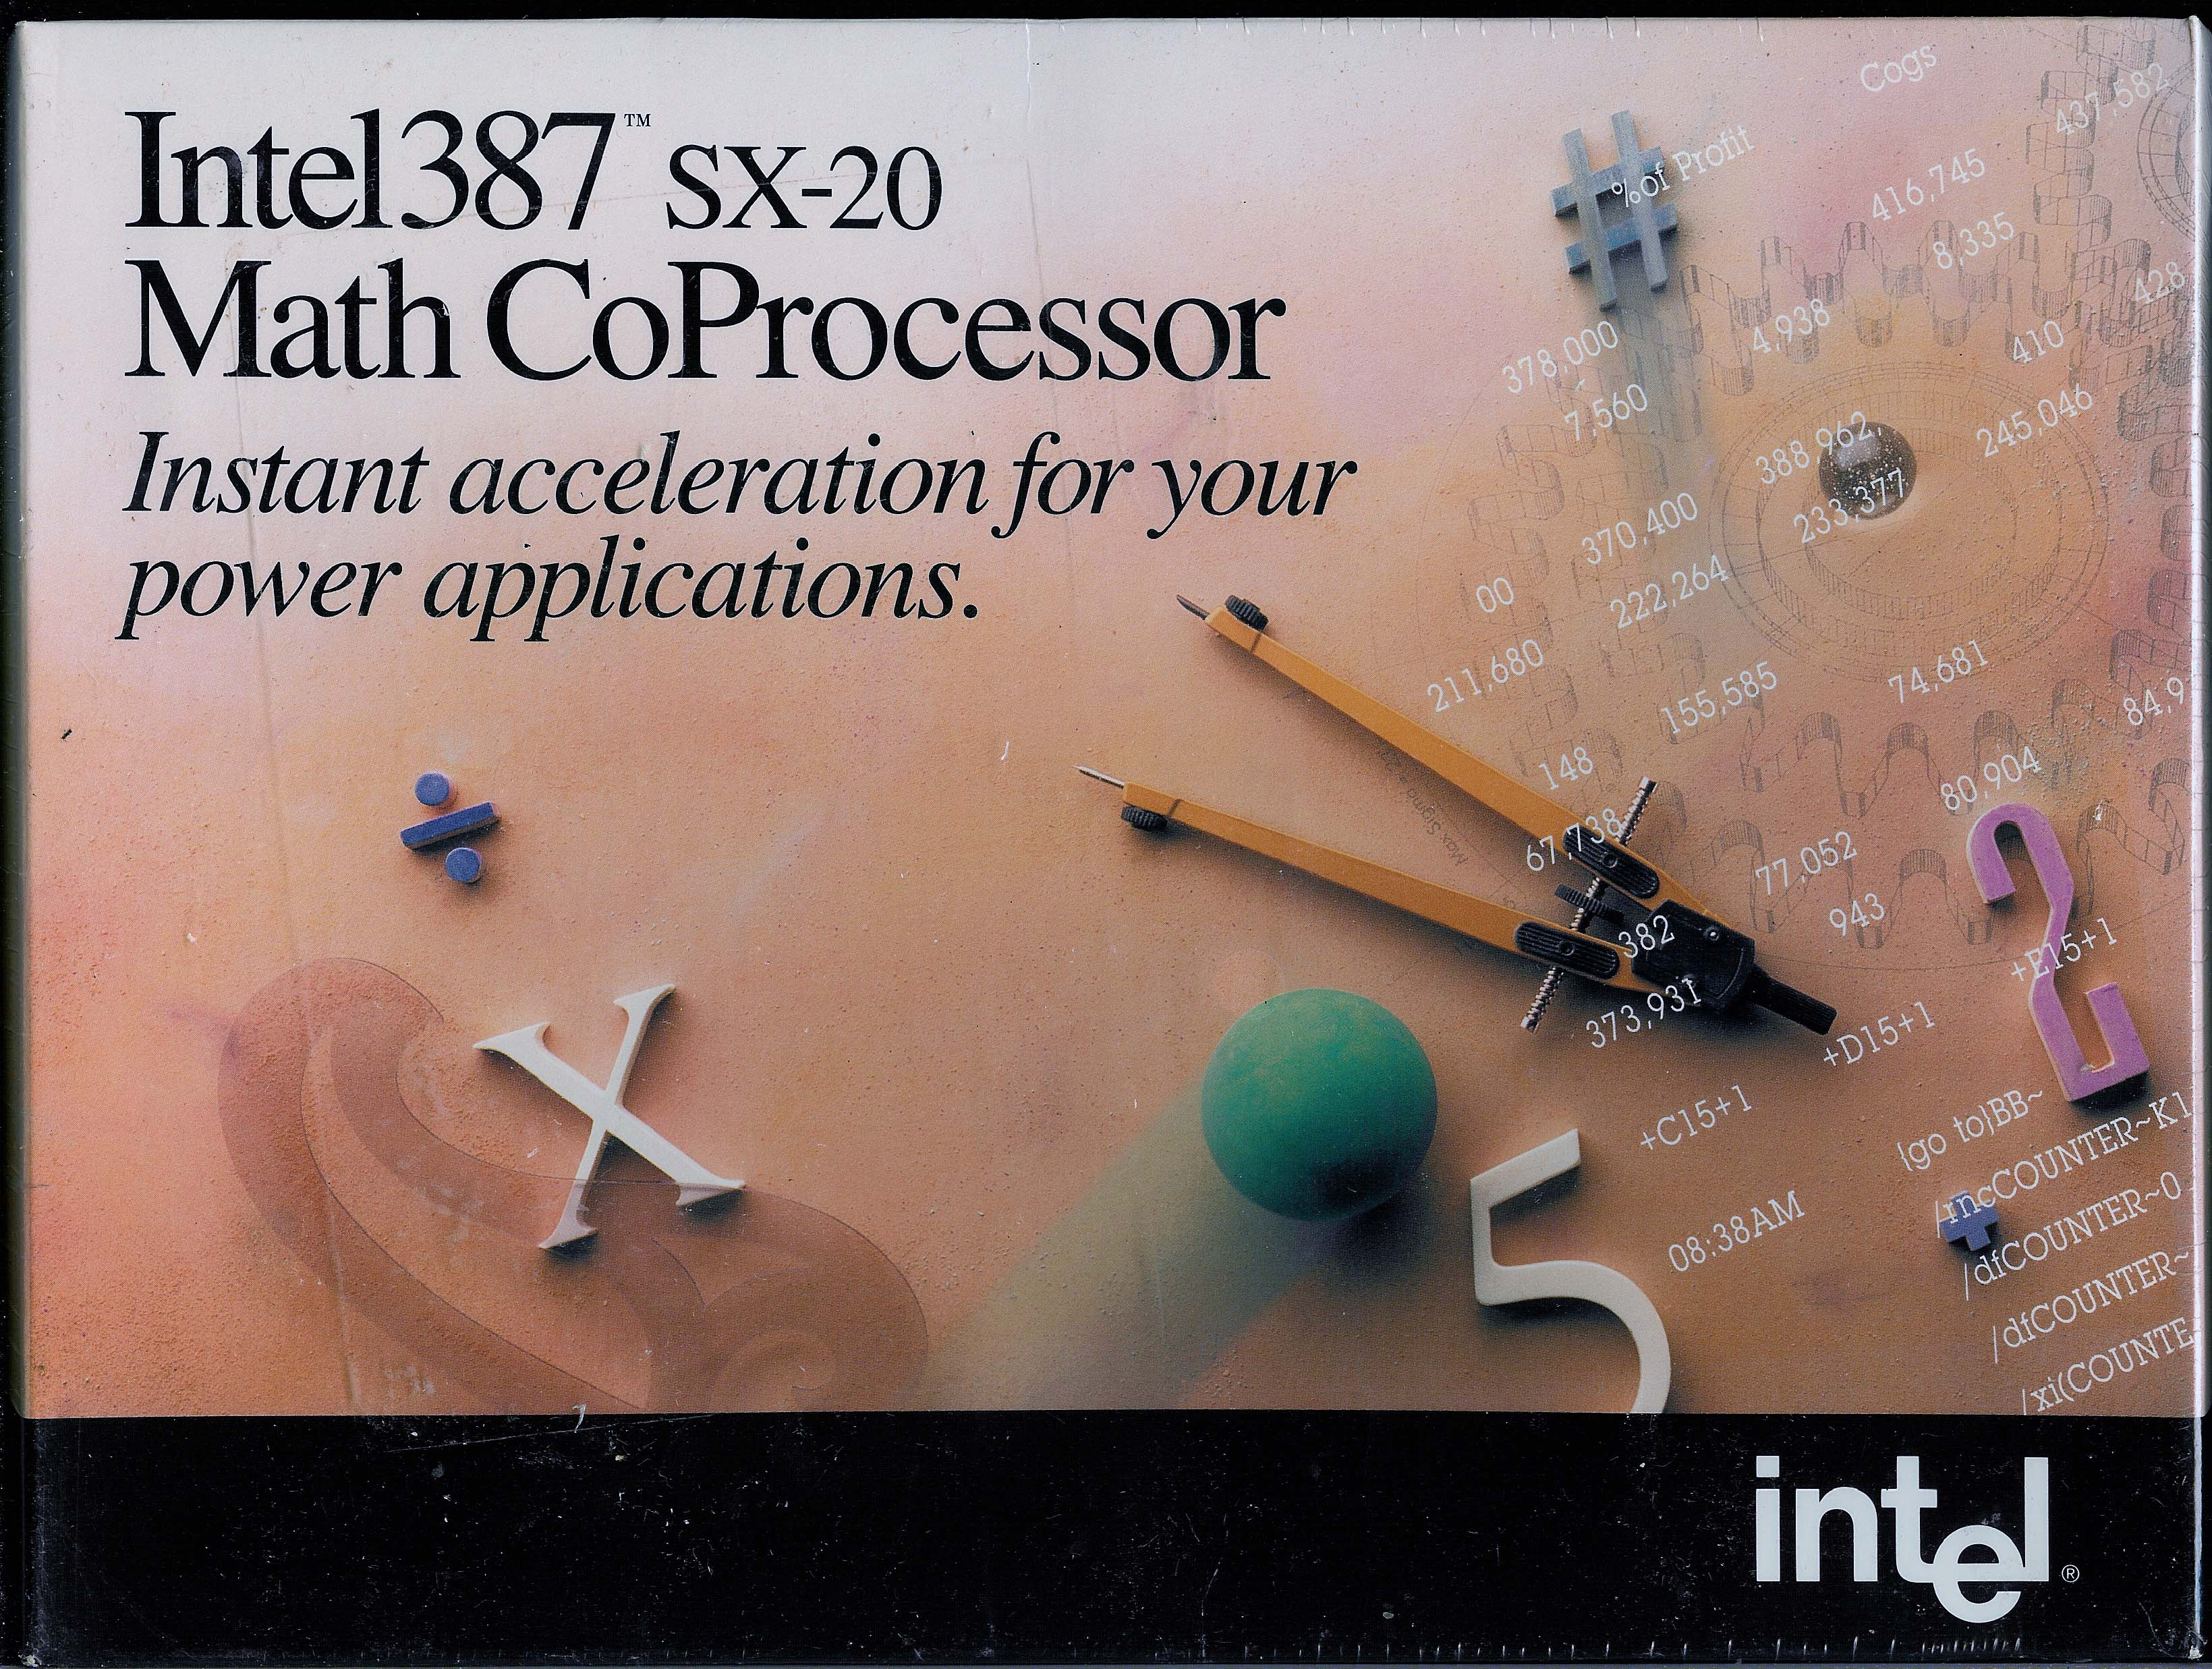
\includegraphics[scale=0.5]{imgs/BOX_IntelBOX387SX20.jpg}
  }
\caption{Intel 1991 ad for "Math CoProcessor".}
\label{fig:fp_internals}
\end{figure}



\bigskip
Overall the CPU was not promising for a 3D game: 286 and 386 \emph{int} operations were fast but not accurate enough and \emph{float} operations were accurate but not fast enough.
   















\section{RAM}
Intel CPUs could operate in two modes:
\begin{itemize}
  \item The old backward compatible Real Mode. Available \emph{only} to allow old software to run. This memory model replicated how the Intel 8086 CPU from the 70s operated: 20 bits memory bus, 1MB addressable RAM with an awful segmented addressing system.
  \item The new Protected Mode with a 32 bits memory bus wide offering up to 4 GB of RAM protectable with a MMU\footnote{Memory management Unit}.
\end{itemize}
The machine started in Real Mode for compatibility reasons. You may assume that programers of the 90s switched the CPU in Protected Mode to unleash the full potential of the machines and ditch the 20 years old Real Mode. Unfortunately, there was a major obstacle between this nice feature and the programmer. The infamous operating system, MS-DOS 5.0 by Microsoft Corporation.
  






  \subsection{DOS limitations}
  Microsoft Corporation highly valued the applications running on their operating systems. They were adamant to never ever break anything with a new system.  Since many applications were written during the 80s on machine having only Real-Mode, DOS 5.0 kept running that way and as a result its routines and system calls were incompatible with Protected Mode. This created an awkward situation where the \emph{de-facto} operating system that came with every machine sold prevented programmers from using Protected Mode. They were forced to ignore all the neat features of their 1992 PC and use the machine like it was a very fast Intel 8086 CPU from 1976.

\bigskip

 \textbf{\underline{Trivia :}} One year earlier, in 1991, a student from the University of Helsinki started working on a "hobby" of his: An operating system able to use the CPU in Protected Mode taking advantage of the MMU and the 32 bits registers. It would become Microsoft worse nightmare. Linus Torvalds had just started what would become Linux.



  \subsection{The infamous Real Mode: 1MB RAM max}
  Protected mode was unavailable. What had the Real-Mode to offer ? Essentially a trip back in time to 1976: A 20 bits wide address bus offering only 1MB of addressable RAM. No matter how much memory was installed on the machine in 1992, only 1MB could be addressed. And to top it all, addressing had to be done not with the 32 bits registers available but by combining two 16 bits register together: One was the segment, the other an offset within that segment. Hence the name: '16 bits programming'.

  \bigskip
Here is a brief description of the memory layout: \\
\begin{itemize}
\item From 00000h to 003FFh : the Interrupt Vector Table.
\item From 00400h to 004FFh : BIOS data.
\item From 00500h to 005FFh : command.com+io.sys.
\item From 00600h to 9FFFFh : Usable by a program (around 620KB). 
\item From A0000h to FFFFFh : UMA (Upper Memory Area): Reserved to bios ROM, video card and sound card mapped I/O.
\end{itemize}

\begin{figure}[H]
\centering
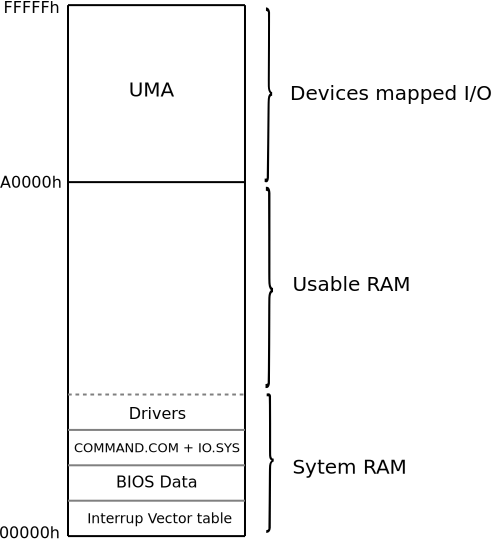
\includegraphics[scale=1]{imgs/real_mode.pdf}

\caption{3.14 window and offset.}
\label{fig:fp_internals}
\end{figure}


As a result, out of the original 1024KB, only 640KB (called Conventional Memory) were usable. 384KB were reserved for the UMA\footnote{Upper Memory Area} and every single driver installed (\codeword{.SYS} and \codeword{.COM})  took away from the remaining 640KB.

\bigskip

\textbf{\underline{Trivia :}}  In France people had to load KEYBFR.SYS driver so their AZERTY keyboard keys woud be properly mapped. The driver consumed a whopping 5KB of Conventional Memory.\\
\\

\subsection{The infamous Real Mode: 16 bits Segmented addressing}
Real Mode could not use 32 bits registers for addressing. Everything had to be done by combining two 16 bits registers as seen in Figure \ref{fig:register_comb_to_20_bits}. There were two kinds of RAM pointers: near and far. In the case of a far pointer, a 16 bits segment register would be shifted left 4 bits and combined with an other 16 bits offset register\\
\begin{figure}[H]
\centering
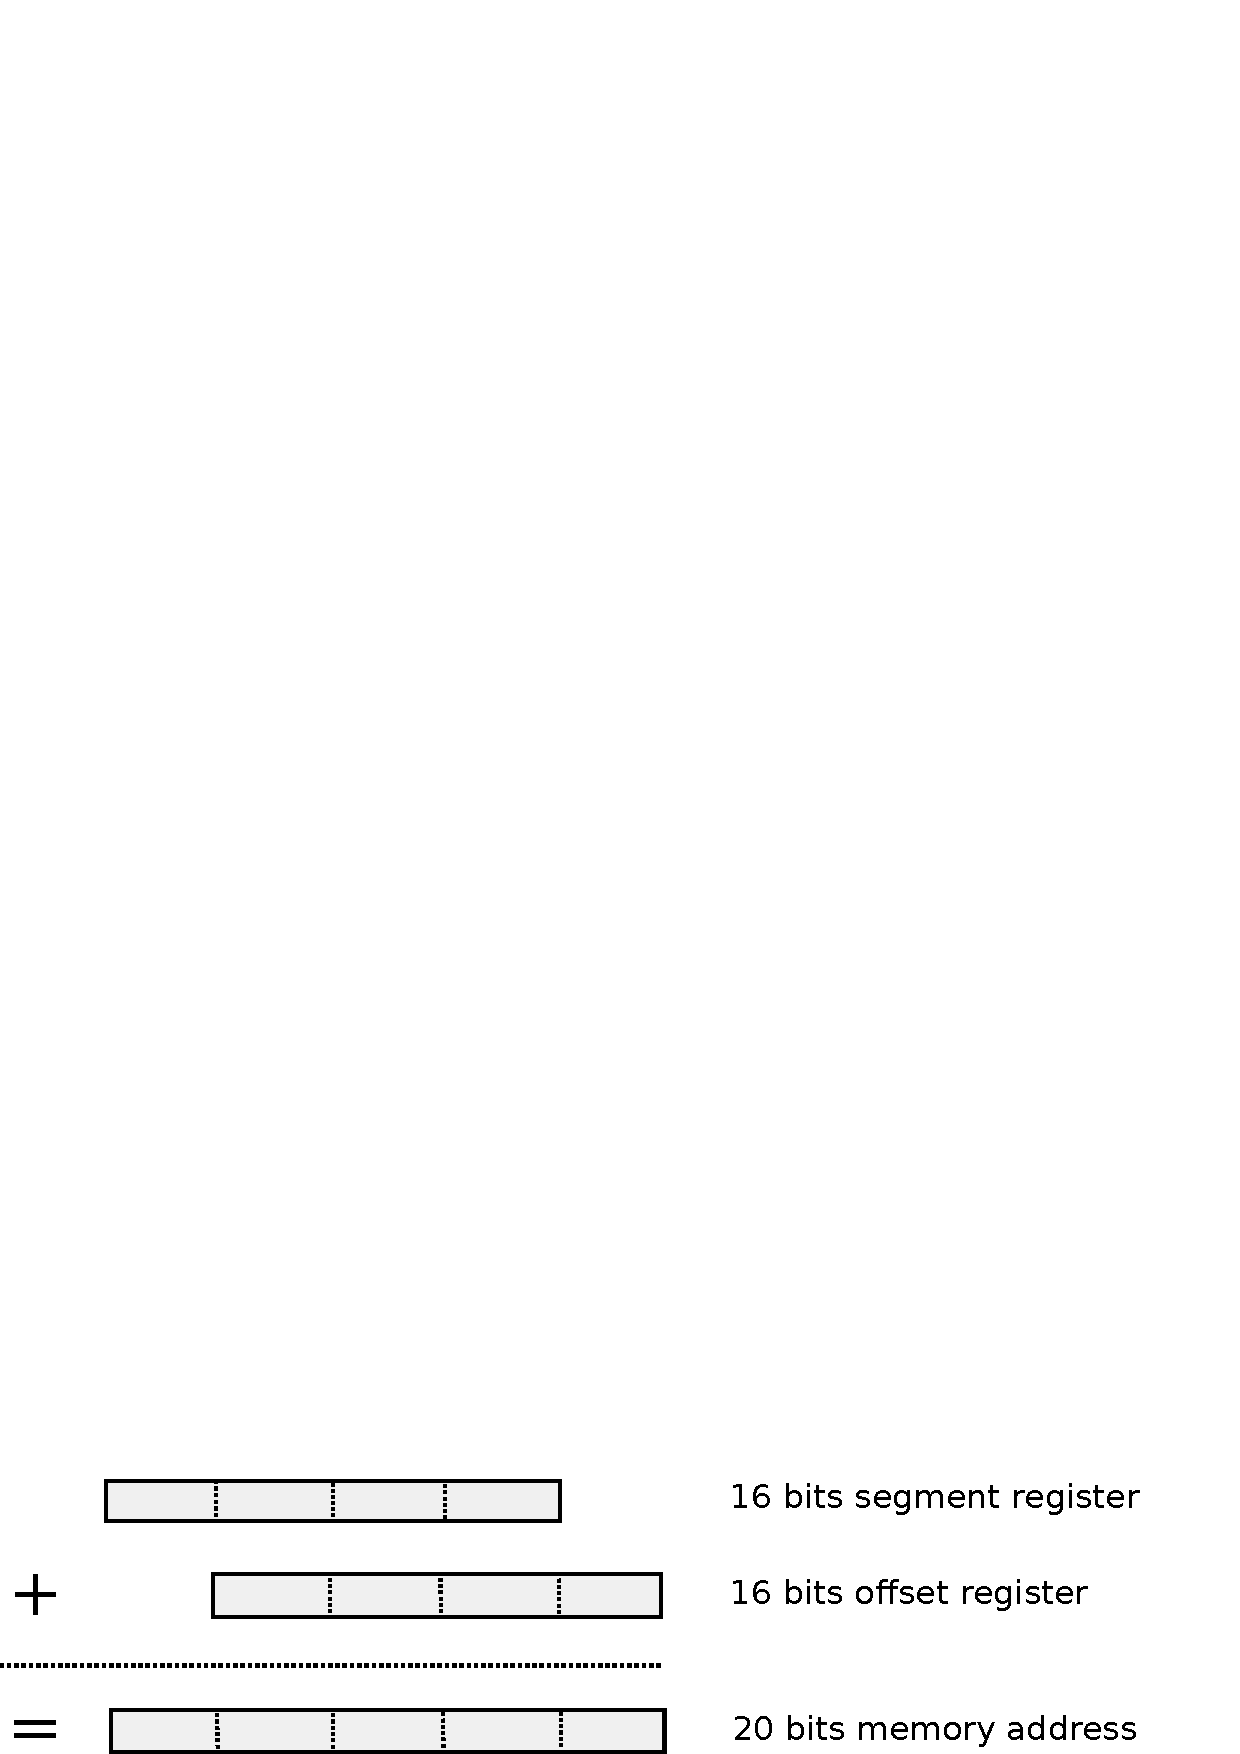
\includegraphics[scale=0.8]{imgs/register_combination_20_bits_address.pdf}
\caption{How registers were combined to address memory.}
\label{fig:register_comb_to_20_bits}
\end{figure}
A near pointer was just a 16 bits offset that would point in the same segment. 
\bigskip
That may not sound too bad but in practice this segmented addressing led to many issues.
The least problematic was about the language: Since the C language was invented on 32 bits machine, the language had to be augmented by compiler manufacturers. That is how the \codeword{near} and \codeword{far} keywords came to existence. To build pointers, a set of macro would be provided, respectively \codeword{FP\_SEG} and \codeword{FP\_OFF}. That was an ugly wart on the beautiful C but that was manageable.\\
\\
The really big issue however was how two pointers, referring to the same address could fail an equality test: In this model, the 1MB of RAM is divided in 65536 paragraphs by the segment pointer. So a paragraph is 16 bytes but an offset can be up to 65536 !!! See the following example:\\
\bigskip
\\Pointer A defined as:
\begin{Verbatim}[fontsize=\relsize{-1}]
    0000 0000 0000 0000 0000  Segment, 16 bits shifted 4 bits left  
  +      0000 0001 0010 0000  Offet,   16 bits
============================
    0000 0000 0001 0010 0000  Address, 20 bits
\end{Verbatim}

\bigskip

Pointer B defined as:
\begin{Verbatim}[fontsize=\relsize{-1}]
    0000 0000 0001 0000 0000  Segment, 16 bits shifted 4 bits left  
  +      0000 0000 0010 0000  Offet,   16 bits
============================
    0000 0000 0001 0010 0000  Address, 20 bits
\end{Verbatim}

\bigskip

Pointer C defined as:
\begin{Verbatim}[fontsize=\relsize{-1}]
    0000 0000 0001 0010 0000  Segment, 16 bits shifted 4 bits left  
  +      0000 0000 0000 0000  Offet,   16 bits
============================
    0000 0000 0001 0010 0000  Address, 20 bits
\end{Verbatim}

As defined A, B and C all points to the same memory location however they would fail a comparison test in the following code.\\

\lstinputlisting[language=C]{code/pointer_madness.c}

Woud output:


\lstinputlisting{code/pointer_madness_output.txt}

\bigskip





  \subsection{Extended Memory}

The 20 bits address bus of Real Mode limited the addressable RAM to 1MB. But machines of 1992 came equipped with more, typically 2MB and even sometimes 4MB. The workaround at the time was to install special drivers that would open a window beyond the addressable RAM as shown in Figure \ref{fig:ems_xms_layout}.

\begin{figure}[H]
\centering
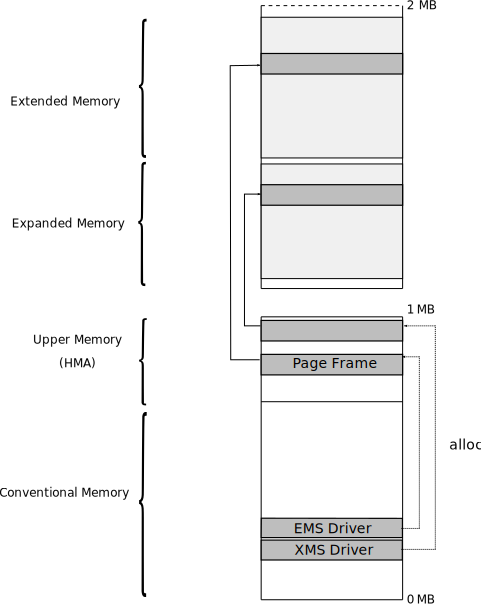
\includegraphics[scale=1]{imgs/expanded_ram}
\caption{Expanded memory layout}
\label{fig:ems_xms_layout}
\end{figure}
With this system, programmer could map part of the upper memory to RAM located beyond the addressable space.
Unfortunately once again, nothing was standardized. Users could load different drivers providing different memory mapping systems:
\begin{itemize}
\item Expanded Memory Specification (EMS) drivers: EMM368.SYS.
\item eXtended Memory Specification (XMS) drivers: HIMEM.SYS .
\end{itemize}

Or they could decide to load no drivers at all at startup and not use any of the RAM beyond 1MB.\\
\textbf{\underline{Trivia :}}  This 640KB barrier was a big issue. Many customer could not understand why even though they had many MB installed on their machine, some game would refuse to start up claiming "Not enough memory". id Software had to publish an explanation (Appendix "\nameref{chap:barrier640}") along with the game to make it clear that it was not their fault.\\

\textbf{\underline{Trivia :}}  As of 2014, thirty five years after the introduction of the 8086, most PC in the world still start in Real Mode. A bootloader switch them to protected mode, load the kernel and then real startup can begin. Mac computers don't have this problem.

\bigskip

TODO: Include reference to XMS and EMS programming reference. \footnote{eXtended Memory Specification (XMS) July 19, 1988.}\\

TODO: Include starting screen of Wolf3D showing available memory.\\

\section{Video}

PC were connected to CRT monitors: Big, heavy, small diagonal, cathodic ray based with curved surface screens. Most monitors had a 13" diagonal with a 4:3 aspect ratio. Figure \ref{fig:int_layout} shows a comparison between a 13" CRT from 1992 and a 28" LCD display from 2014.\\

\begin{figure}[H]
\centering
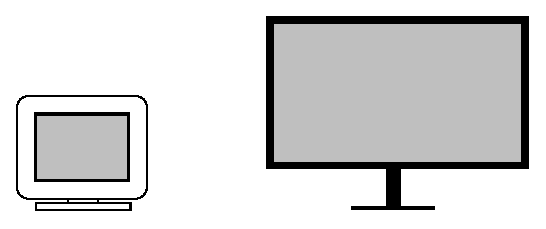
\includegraphics[scale=1.2]{imgs/crt_lcd.eps}
\caption{CRT (left) vs LCD (right)}
\label{fig:lcd_vs_crt}
\end{figure}

\textbf{\underline{Trivia :}} How big and heavy could a CRT be ? The InterView 28hd96 by Integraph weighted 45kg (99.5lb). For comparison, a modern DELL LCD 27" weights 7.8kg (17lb).\\
\\
The main issue in this system is that CRT are analogic system while computers are digital. An interface system is needed between the two and it came as a serie of chipsets called "Adapters".

  \subsection{History}

The first adapter of the family was released in 1981. The Monochrome Display
   Adapter (\codeword{MDA}) was monochrome with low resolutions but it had the merit to be on every PC sold. Many other systems followed over the years, always preserving backward compatibility like it was the tradition at the time:
\bigskip
  
 \begin{figure}[H]
\centering  
\begin{tabularx}{0.9\textwidth}{ X  Y }
  \toprule
  \textbf{Name} &  \textbf{Year Released} \\
  \toprule \codeword{MDA}
   (\textbf{M}onochrome
   \textbf{D}isplay
   \textbf{A}dapater) & 1981 
   \\ \codeword{CGA}
   (\textbf{C}olor
   \textbf{G}raphics
   \textbf{A}dapter) & 1981 
    \\ \codeword{EGA}
   (\textbf{E}nhanced
   \textbf{G}raphics
   \textbf{A}dapter) & 1985
   \\ \codeword{VGA}
   (\textbf{V}ideo
   \textbf{G}raphics
   \textbf{A}rray)  & 1987
    \\
  \toprule
\end{tabularx}
\caption{Video interface history.}\label{fig:vga_history}
\end{figure}

Each iteration added new features and in 1993 the ubiquitous graphic system was the VGA\footnote{Video Graphic Adapter}. The universality of that system was a two edged sword: One one side developers had to program for one graphic system only. But on the other side, there was no escape to the shortcoming of the Adapter (and people did not purchase separate GPU back then).\\

\subsection{VGA Architecture}

The VGA can be summarized as two major systems :

\begin{itemize}
\item The Graphic Controller and Sequence Controller controlled how the VGA RAM was accessed (interface CPU-VRAM).
\item The framebuffer (VGA RAM) made not of one memory bank of 256KB but four memory banks of 64KB.
\item The CRTC Controller and the DAC (Digital To Analog Converter) took care of converting the Palette indexed framebuffer to RGB and then to analogic signal (interface VRAM-CRT).
\end{itemize}

The most surprising part of the architecture is obviously the framebuffer. The first reaction of any engineer would be to ask themselves: Why four banks instead of one clean big one ?\\
\\
The first part of the explanation comes from backward compatibility: The version before VGA, the EGA had only 64KB of RAM. It was very easy to design a backward compatible system that used only one bank of 64KB.\\
\\
But the real reason was physical limitations: A CRT running at 60Hz and displaying 640x480 needed a pixel every 1/(640*480*60)th of a second . That means one pixel each 54ns. The problem was that RAM access time was 200ns: Not nearly fast enough\footnote{Computer Graphic: Principles and Practice 2nd Edition, page 168} to refresh the screen at 60hz. If latency could not be reduced, the throughput could still be improved by accessing four banks at the time. The memory banks read in parallel had an amortized latency of 200/4 = 50ns/pixel which was fast enough.


\begin{figure}[H]
\centering
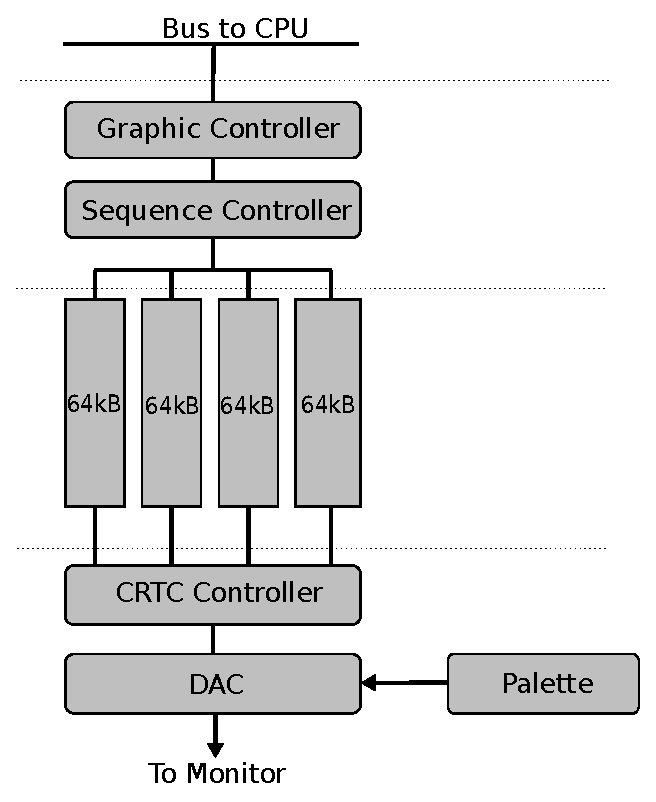
\includegraphics[scale=1.2]{imgs/vga.eps}
\caption{Video Graphic Array Architecture.}
\label{fig:vga_arch}
\end{figure}




\subsection{VGA Planar madness}

Four memory banks granted enough throughput to reach high resolutions. The price was complexity of programming aknowledged by even the best programmers of the time:\\

 \begin{fancyquotes}
   Right off the bat, I'd like to make one thing perfectly clear: The VGA is hard-sometimes very hard-to program for good performance.
 \bigskip \\
\textbf{Michael Abrash - Graphic Programming Black Book}
 \end{fancyquotes}
 \\
\bigskip
My first drawing of the VGA was actually deceiving. It was a hell of a system to work with. The diagram from IBM VGA Reference illustrate this pretty well:\\
 \begin{figure}[H]
\centering
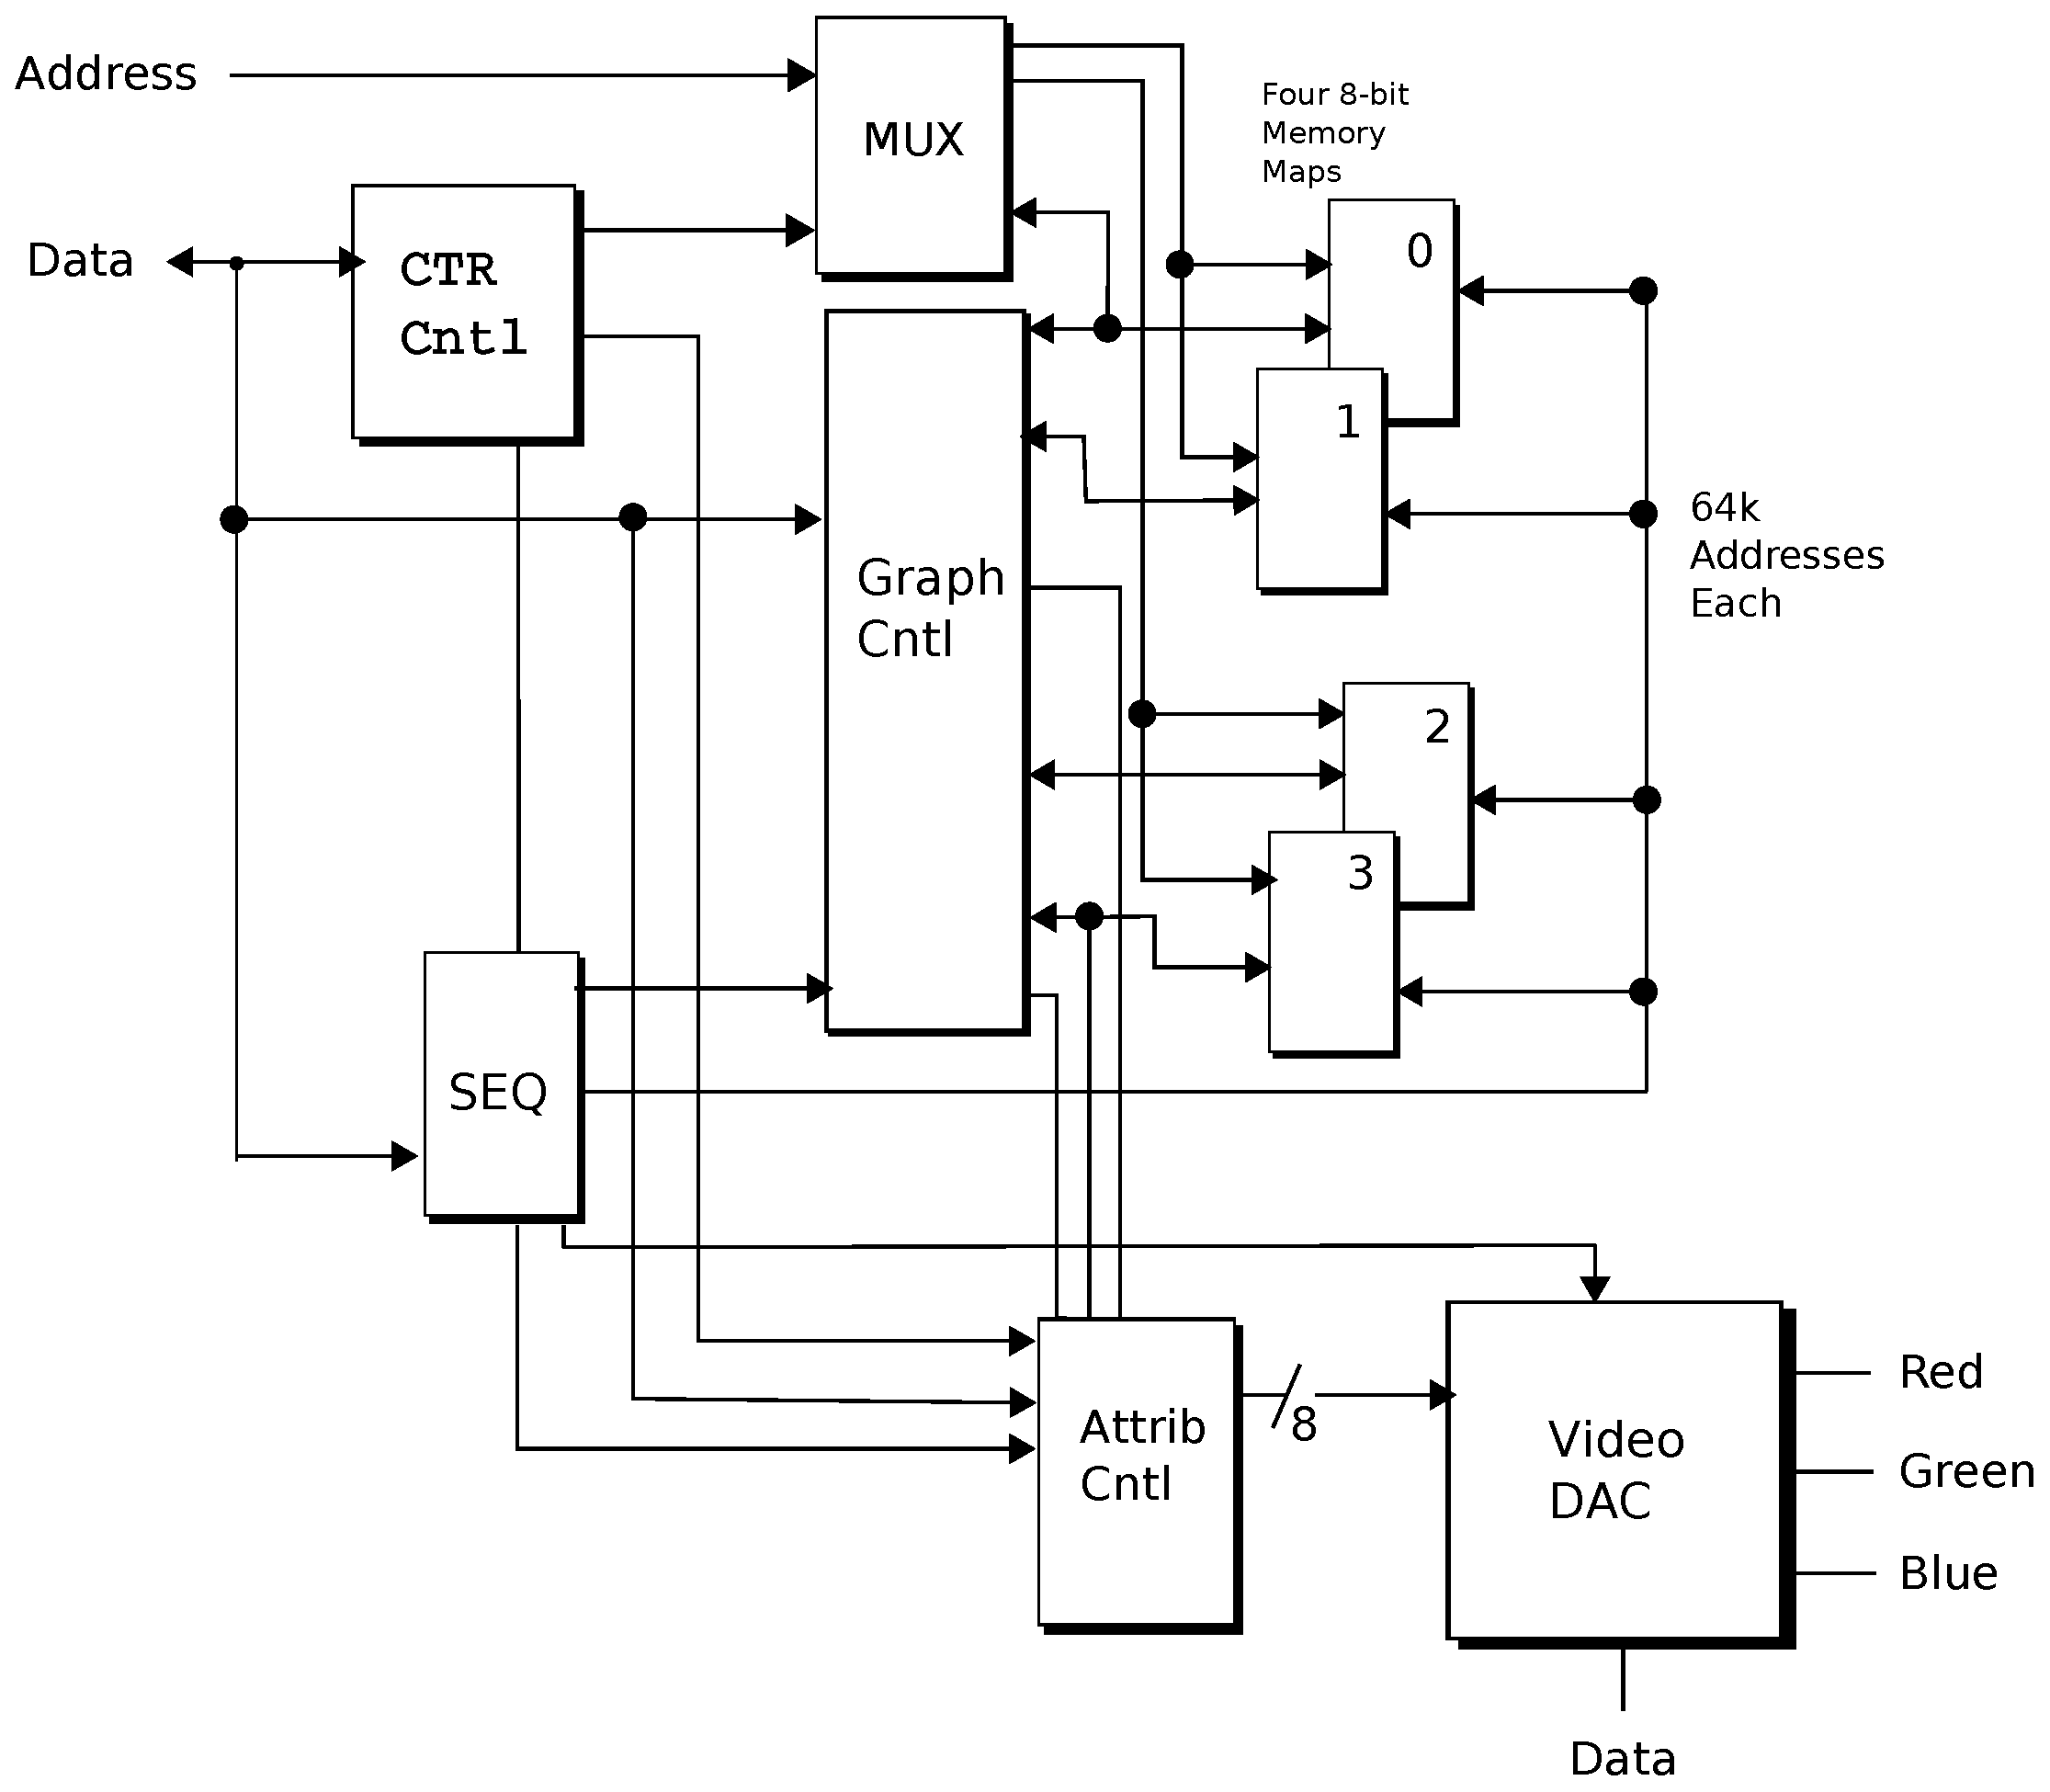
\includegraphics[scale=0.38]{imgs/ibm_vga.eps}
%\def\svgscale{1.5}
%\input{imgs/fun_pipeline.pdf_tex}
\caption{IBM's VGA Documentation}
\label{fig:ibm_vga}
\end{figure}

\bigskip

How memory banks were populated vs how they were displayed:
\begin{figure}[H]
\centering
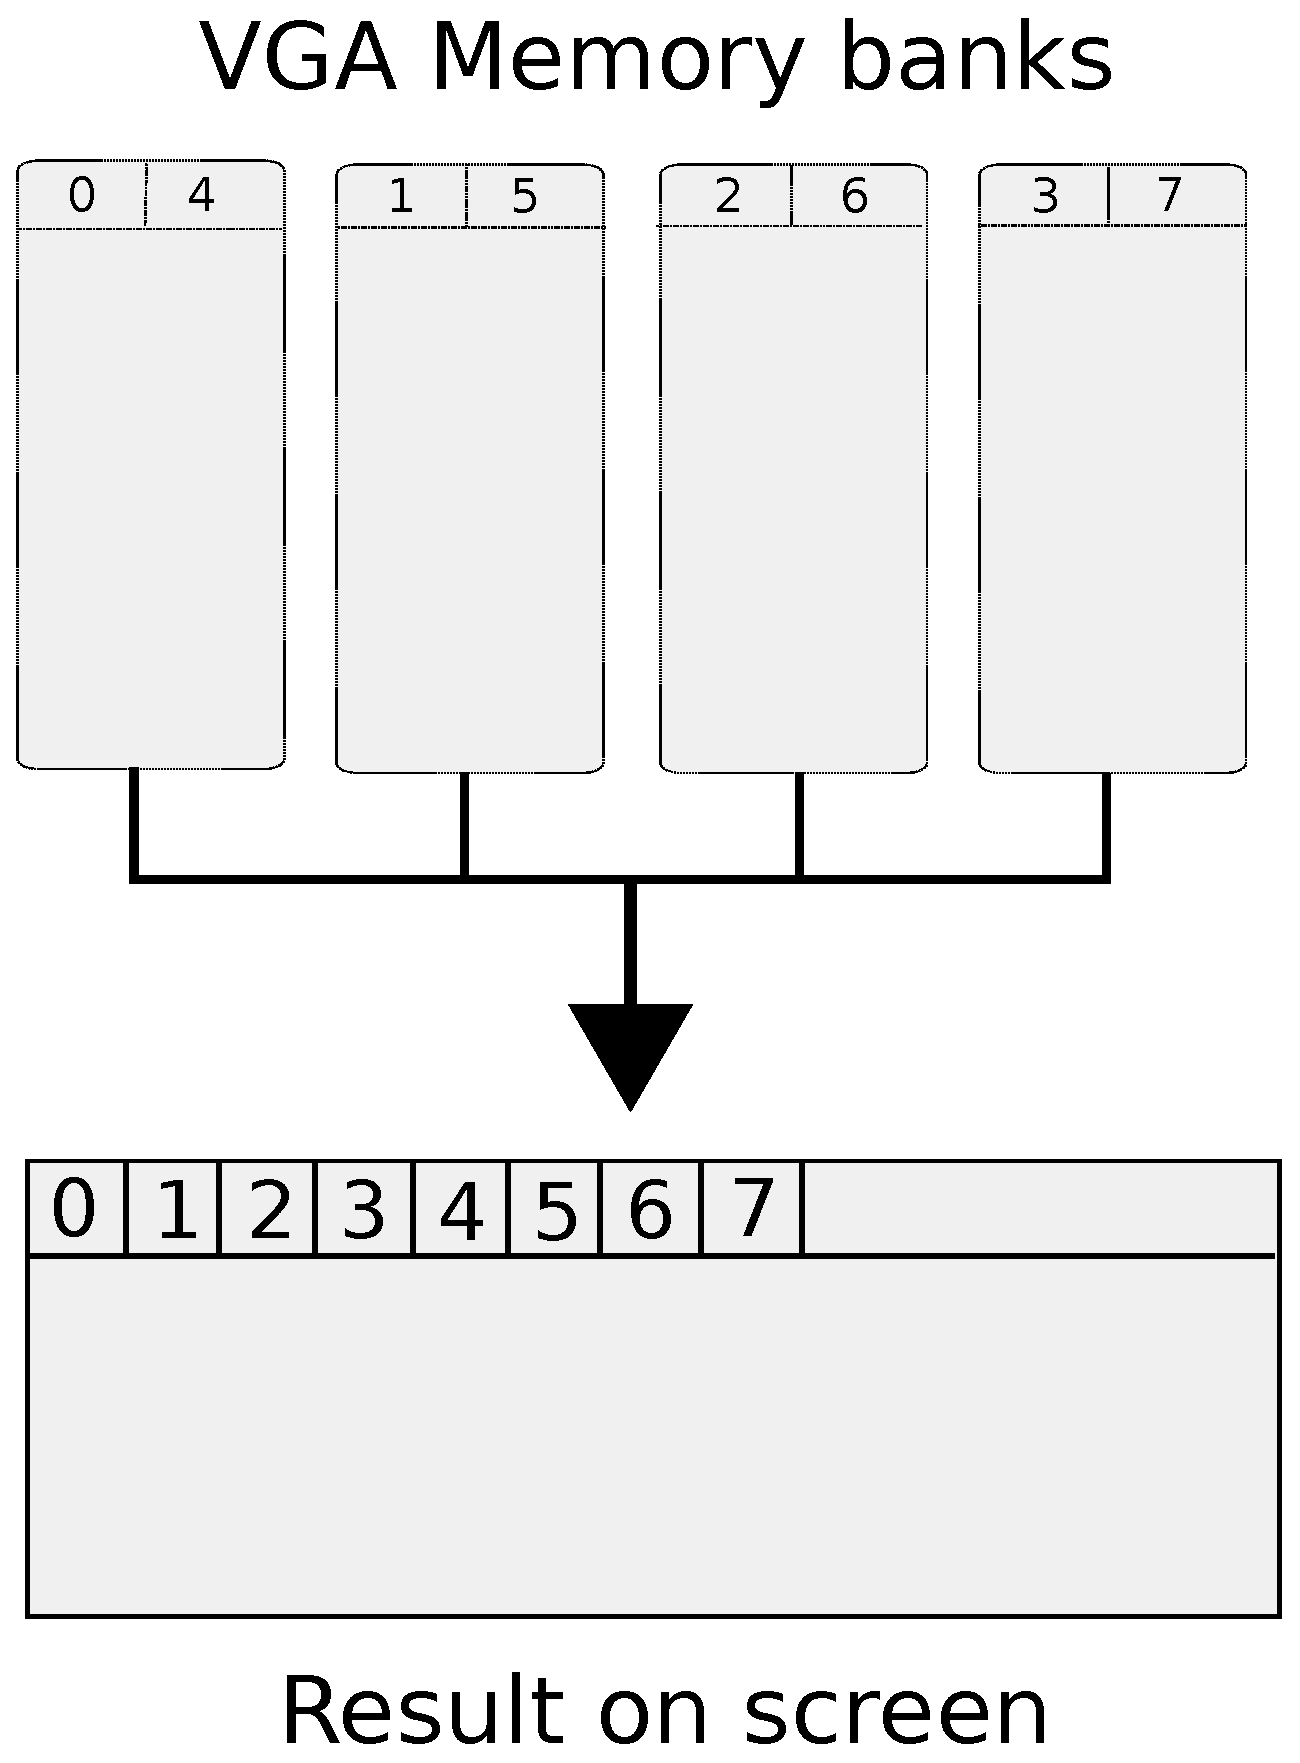
\includegraphics[scale=0.5]{imgs/vga_ram_screen_layout.eps}
\caption{Video Graphic Array Architecture.}
\label{fig:vga_arch}
\end{figure}
 
\bigskip
To configure this mess of planes, registers and controllers meant setting up more than 300 poorly documented registers to interact together. Needless to say few programmers got to dive in the internal of this thing. Luckily IBM BIOS had a few preset configuration (called "mode") with an associated resolution and color numbers.

\subsection{VGA Modes}

The BIOS could be called to have the VGA configured with preset registers.

\begin{figure}[H]
\centering
\begin{table}[H]
\begin{tabular}[c]{llllr}
\hline
\textbf{Mode} & \textbf{Type} & \textbf{Format} & \textbf{Colors}          & \multicolumn{1}{l}{\textbf{Segment}} \\ \hline
0             & text          & 40x25           & 16 gradient (monochrome) & b800h                                \\ \hline
1             & text          & 40x25           & 16                       & b800h                                \\ \hline
2             & text          & 80x25           & 16 gradient (monochrome) & b800h                                \\ \hline
3             & text          & 80x25           & 16                       & b800h                                \\ \hline
4             & CGA Graphics  & 320x200         & 4                        & b800h                                \\ \hline
5             & CGA Graphics  & 320x200         & 4 gradient (monochrome)  & b800h                                \\ \hline
6             & CGA Graphics  & 640x200         & 2                        & b800h                                \\ \hline
7             & MDA text      & 9x14            & 3 gradient (monochrome   & b000h                                \\ \hline
0Dh           & EGA graphic   & 320x200         & 16                       & A000h                                \\ \hline
0Eh           & EGA graphic   & 640x200         & 16                       & A000h                                \\ \hline
0Fh           & EGA graphic   & 640x350         & 3                        & A000h                                \\ \hline
10h           & EGA graphic   & 640x350         & 16                       & A000h                                \\ \hline
11h           & VGA graphic   & 640x480         & 2                        & A000h                                \\ \hline
12h           & VGA graphic   & 640x480         & 16                       & A000h                                \\ \hline
13h           & VGA graphic   & 320x200         & 256                      & A000h                                \\ \hline
\end{tabular}
\end{table}
\caption{VGA Modes available from BIOS.}\label{fig:vga_modes}
 \end{figure}
 
 Programmers referenced VGA modes by their ID. It was a common thing to see tutorial about Mode 12h or Mode 13 which were the two most appealing mode for game programming.


 
 



 
 
  \subsection{VGA Programming: Mode 13h}
  Using the VGA as per the manual is easy since two instructions are enough to ask the BIOS to setup the environment with a mode. Here is an example that setup the a VGA to operate at 320x200 with 256 indexed colors: Mode 13h.\\
  \lstinputlisting[ language={[x86masm]Assembler}]{code/vga_mode13.asm}
  
  
  Two instructions and that is it. The \codeword{int 10} is a software interrupt call to the BIOS routine in charge of Graphic setup. It looks up the \codeword{ax} register to setup all 300 VGA register with the corresponding mode.\\
  
  A convenient thing with those was how the four memory banks were hidden to the programmer. By using 2 bits from the RAM, the VGA automatically determined in which bank to store a value. The side effect was to waste 75\% of the RAM. Memory Mapped area:\\
  DRAWING
  
  The programmer has access to a linear framebuffer of 64KB mapped at \codeword{A0000h}.\\
  
  DRAWING
  
  To clear the screen to black for example, the following code was enough:\\
  
  \lstinputlisting[language=C]{code/clear_vga.c}
  
  
  The mode 13h may look good but it is in fact terrible for game and animation. The intend was clearly to display static images:
  \begin{itemize}
\item All the RAM is used and there is no way to have a double buffer.
\item Since the resolution is 320x200, the aspect ration does not feet the monitor. As a result the image is streched when transfered from the 
framebuffer to the CRT.

 \begin{figure}[H]
\centering
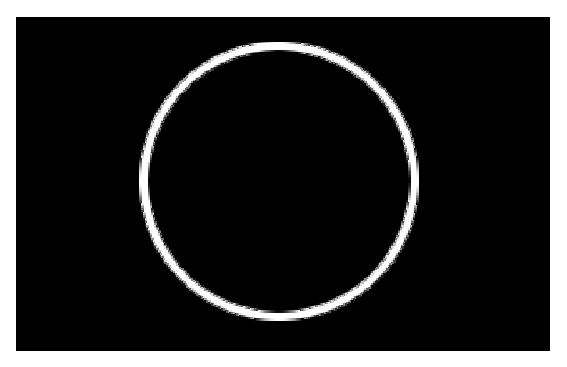
\includegraphics[scale=1.0]{imgs/circleframebuffer.eps}
%\def\svgscale{1.5}
%\input{imgs/fun_pipeline.pdf_tex}
\caption{Drawing a circle in the framebuffer}
\end{figure}

 \begin{figure}[H]
\centering
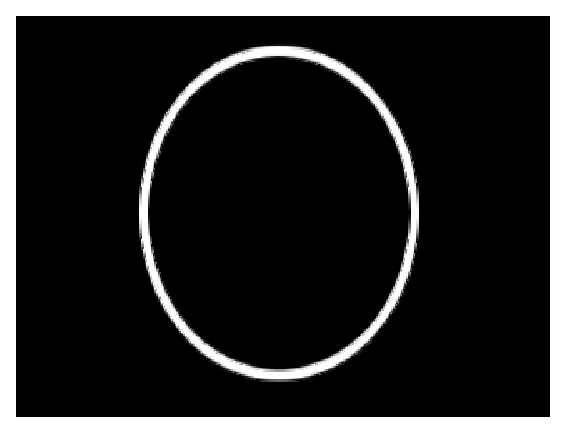
\includegraphics[scale=1.0]{imgs/circlescreen.eps}
%\def\svgscale{1.5}
%\input{imgs/fun_pipeline.pdf_tex}
\caption{How the framebuffer looked once streshed on the CRT monitor :( !}
\end{figure}

\item VGA MAPPING I/O WASTED SPACE.

\end{itemize}

\subsection{What VGA meant for games}
Not sprite engine meant a full framebuffer was had to be populated for any type of animation.\\
Off all parts of the system, the VGA was in appearance the weakest of them all. Single-handedly preventing any type of smooth, tearless animation.




  

\section{Audio}
Off all the parts in a PC, the audio system was the best. The card manufacturer had started to see a market and player actually had the opportunity to buy decent extension "sound card" from Ad Lib or SoundBlaster.
  \subsection{Speaker}
  PC came out of the box with a binary beeper. It was capable to produce two frequencies with surprisingly good results such as in Monkey Island game.\footnote{https://www.youtube.com/watch?v=a324ykKV-7Y}
  \subsection{Ad Lib}
  Ad Lib was a Canadian manufacturer of sound cards. As early as XXXX they identified the limitations of the PC Speakers and started to manufactur a card to connect othe ISA bus. Allowd MIDI.
  
  Note: Canadian company and especially from Quebec were very innovative in the early 90s. Ad Lib manufactured Sound Card, Matrox made a killing with Millenium Graphic Card, Watcom compiler, ATI.\\
  
  Music (midi)
  Not about canada: adlib, watcom and matrox millenium
  \subsection{Sound Blaster}
  The Sound Blaster 1.0 (code named "Killer Kard"),[1] CT1320A, was released in 1989
  Music (midi+digitized sound)]  But it also added two key features absent from the Adlib: a PCM audio channel, and a game port.
  \subsection{Sound Blaster Pro}
  Model CT1330, announced in May 1991, was the first significant redesign of the card's core features, and complied with the Microsoft MPC standard.[6]. The Sound Blaster Pro supported faster digital sampling rates (up to 22.05 kHz stereo or 44.1 kHz mono), added a "mixer" to provide a crude master volume control (independent of the volume of sound sources feeding the mixer), and a crude high pass or low pass filter. The Sound Blaster Pro used a pair of YM3812 chips to provide stereo music-synthesis (one for each channel).
\section{Inputs}
Even though it is anecdotic I still wanted to write a part about the connectors found on a PC at the time. A time before the ubiquitous USB. In short, inputs were a mess.\\

The parallel port (DB-25) was on every computer and usually used to connect matrix printers (loud thing that printed with aiguilles).
 \begin{figure}[H]
\centering
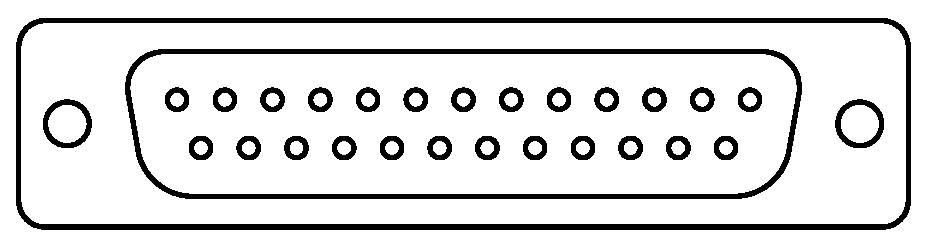
\includegraphics[scale=0.7]{imgs/ports/DB-25_parallel_port.eps}
%\def\svgscale{1.5}
%\input{imgs/fun_pipeline.pdf_tex}
\caption{Parallele Port}
\label{fig:parallelPort}
\end{figure}


The serial port (DE9) was used to connect the mouse.
 \begin{figure}[H]
\centering
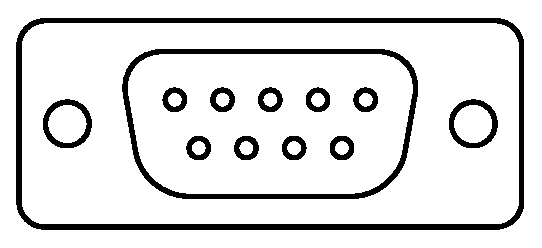
\includegraphics[scale=0.7]{imgs/ports/DE9_serial_port.eps}
%\def\svgscale{1.5}
%\input{imgs/fun_pipeline.pdf_tex}
\caption{Serial Port}
\label{fig:serialPort}
\end{figure}

The PS/2 port was used to connect a keyboard.
 \begin{figure}[H]
\centering
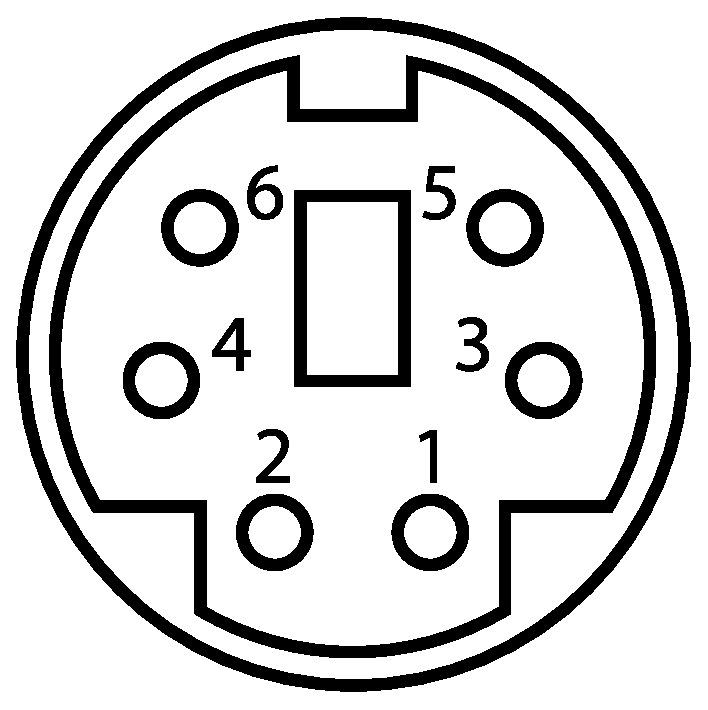
\includegraphics[scale=0.2]{imgs/ports/MiniDIN-6_PS2.eps}
%\def\svgscale{1.5}
%\input{imgs/fun_pipeline.pdf_tex}
\caption{PS/2 Port}
\label{fig:ps2Port}
\end{figure}


Finally, the sound card connected via the ISA bus provided a new port: A Game Port (DA-15) allowing to connect a joystick.
 \begin{figure}[H]
\centering
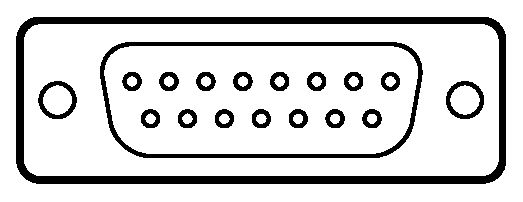
\includegraphics[scale=0.9]{imgs/ports/DA-15_GamePort.eps}
%\def\svgscale{1.5}
%\input{imgs/fun_pipeline.pdf_tex}
\caption{Game Port}
\label{fig:gamePort}
\end{figure}

Note that without a sound card you were unable to connect a joystick !



\section{Summary}

\end{document}




